

%\documentclass[xcolor=dvipsnames,compress,subsection=false,draft]{beamer}
\documentclass[xcolor=dvipsnames,compress,subsection=false]{beamer}
\nonstopmode
\usetheme{Singapore} 
\usepackage{graphicx}
\usepackage{verbatim}
\usepackage{bm}
\usepackage[loop]{animate}
%\usepackage[usenames,dvipsnames,svgnames,table]{xcolor}
%\usepackage[usenames,dvipsnames]{xcolor}
\graphicspath{{assets/}}
\usepackage{xmpmulti}
\usefonttheme[onlymath]{serif}

\title{NetCDF}
\author{Adam M. Wilson}
\date{November 15, 2012}
\setbeamersize{text margin left=6mm, text margin right=6mm} 

\def\slantfrac#1#2{\hbox{$\,^#1\!/_#2$}}

%% show frame number
%\setbeamertemplate{footline}{\scriptsize{\vspace*{0.3cm}\hspace*{0.1cm}\insertframenumber}} 
\setbeamertemplate{navigation symbols}{}%remove navigation symbols
\setbeamerfont{frametitle}{size=\large,series=\bfseries}
\setbeamerfont{alerted text}{series=\bfseries}

\begin{document}

\frame{
  \frametitle{Overview}
Two broad objectives: \\ \bigskip

{\bf Introduction to working with climate data}
 \begin{enumerate}
\item {Explore how the IPCC AR5 data are organized}
\item {Introduce HDF/NetCDF as a data format}
\item {Use Climate Data Operators (CDO) from within R to process the daily data to climate metrics}
\item {Make a few plots}
\end{enumerate}

\\ \bigskip {\bf Illustrate "Literate Programing"}
\begin{enumerate}
\item {Use of R+Markdown to generate repeatable, "human-readable" reports of an analysis.}
\end{enumerate}

}
\section{CMIP5}
\subsection*{}

\frame[t]{
  \frametitle{Coupled Model Intercomparison Project Phase 5 (CMIP5)}
% The CMIP5 experiment design includes the following experiments:
\begin{center}
 \includegraphics<1>[width=.65\textwidth]{CMIP5_1}
 \includegraphics<2>[width=.65\textwidth]{CMIP5_2}
 %   \begin{enumerate}
 %   \item Decadal Hindcasts and Predictions simulations,
%  \item	  "long-term" simulations, 
 % \item   "atmosphere-only" for computationally-demanding models.
  %   \end{enumerate}
   \\  {\tiny  Taylor, et.al., (2012) BAMS 93(4):485--498}.
\end{center}
}

\frame[t]{
  \frametitle{Representative Concentration Pathways (RCP)}
  \begin{center}
%    \begin{itemize}
%    \item Expose 
%    \end{itemize}
   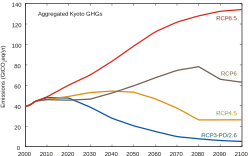
\includegraphics[width=.75\textwidth]{RCP}\\ \bigskip
Plus several historical scenarios (`natural', `green house gases', etc.)
  \end{center}}


\frame[t]{
  \frametitle{Earth System Grid Federation (ESGF)}
  \begin{center}
%    \begin{itemize}
%    \item Expose 
%    \end{itemize}
   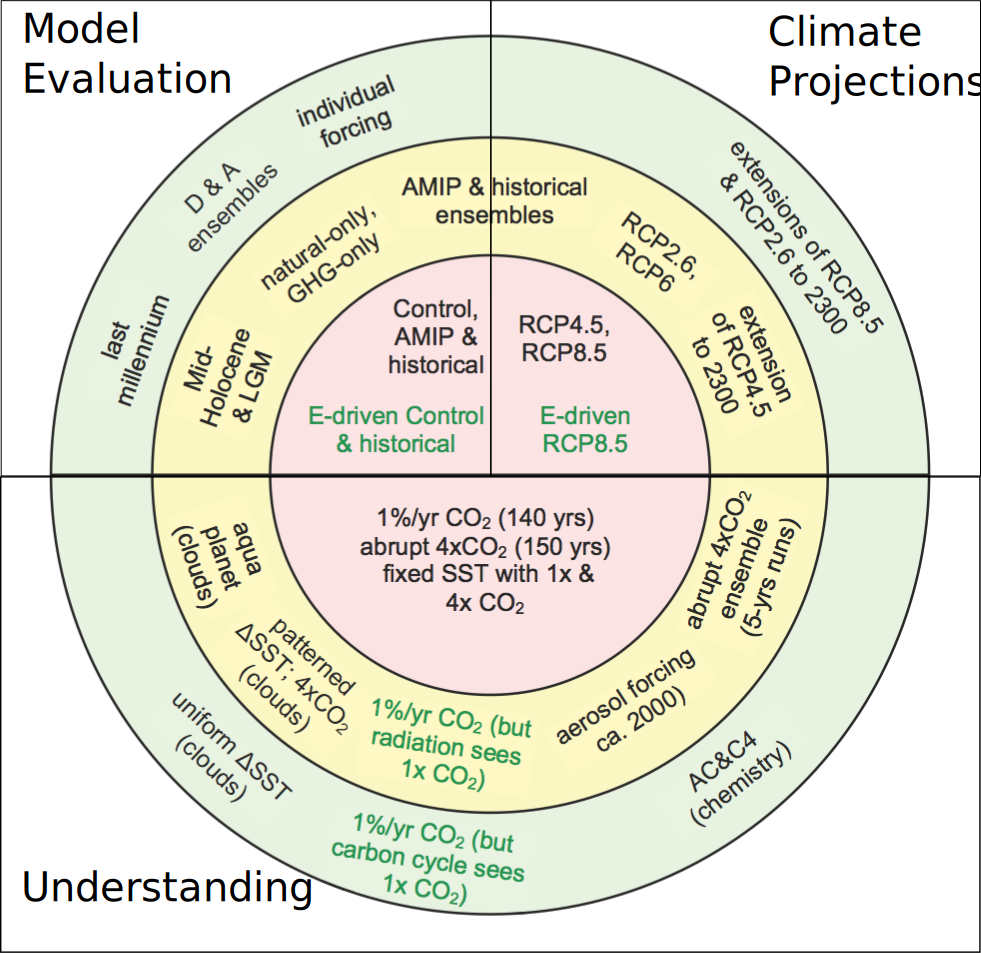
\includegraphics[width=\textwidth]{CMIP5}\\
 \url{http://pcmdi9.llnl.gov/} \\
  Downloads currently not available....
  \end{center}}

\frame[t]{
  \frametitle{Filter via ESGF webpage \url{http://pcmdi9.llnl.gov/}}
  \begin{center}
%    \begin{itemize}
%    \item Expose 
%    \end{itemize}
   \includegraphics[width=.9\textwidth]{ESGF2}\\ \bigskip
  \end{center}}

\begin{frame}[t,fragile]
  \frametitle{ESGF provides a \texttt{wget} script to download the selected data}
  \begin{tiny} 
\begin{verbatim}
#!/bin/bash
###############################################################
# ESG Federation download script
#
# Template version: 1.2
# Generated by pcmdi9.llnl.gov - 2013/10/09 12:02:14
# Search URL: http://pcmdi9.llnl.gov/esg-search/wget/?query=*&
#       dataset_id= cmip5.output1.NOAA-GFDL.GFDL-CM3 \\
#      .rcp85.day.atmos.day.r1i1p1.v20120227|esgdata.gfdl.noaa.gov
#
##############################################################
. . .
version=1.3.2
CACHE_FILE=.$(basename $0).status
openId=
search_url='http://pcmdi9.llnl.gov/esg-search/wget/?query=*&
       dataset_id=cmip5.output1.NOAA-GFDL.GFDL-CM3.rcp85.day.atmos.day.r1i1p1.v20120227| \\
       esgdata.gfdl.noaa.gov'
#These are the embedded files to be downloaded
download_files="$(cat <<EOF--dataset.file.url.chksum_type.chksum
'clt_day_GFDL-CM3_rcp85_r1i1p1_20960101-21001231.nc'
'http://esgdata.gfdl.noaa.gov/thredds/fileServer/gfdl_dataroot/NOAA-GFDL/GFDL-CM3/
rcp85/day/atmos/day/r1i1p1/v20110601/clt/clt_day_GFDL-CM3_rcp85
_r1i1p1_20960101-21001231.nc' 'MD5' '801fc44c406377a084f87c4f509e9da8'
'clt_day_GFDL-CM3_rcp85_r1i1p1_20910101-20951231.nc'
. . . 
  \end{verbatim} 
  \end{tiny}
\end{frame}


\section{Intro to NetCDF}
\subsection*{}

\frame[t]{
  \frametitle{What is NetCDF?}
  \begin{center}
    \begin{itemize}
    \item A netCDF file has named variables,attributes, and dimensions.
    \item  Variables $\rightarrow$ data 
    \item Attibutes $\rightarrow$ metadata (for file or variable)
    \item Dimensions $\rightarrow $ Shapes of variables
    \item  Variables may share dimensions, indicating a common grid
    \item Each variable or attribute $\in$ char, byte, short, int,
      float, double
    \end{itemize}
   \includegraphics[width=\textwidth]{netcdf1.png}\\
  \end{center}}

\frame[t]{
  \frametitle{What is NetCDF?}
  \begin{center}
   \includegraphics[width=.9\textwidth]{netcdf2.png}\\
  \end{center}}

\begin{frame}[t,fragile]
  \frametitle{What is NetCDF?}
  Notation for NetCDF in CDL (Common Data Language)
  \begin{footnotesize} 
\begin{verbatim}
netcdf snow{ 
    dimensions: 
        lon= 9 ; 
        lat= 7 ;
        time = unlimited ;  // 3 currently
    variables:
        float IR\_flux(lon, lat) ;
        IR_flux:units = "W m-2" ;
        IR_flux:_Fill_value = -999 ;
        IR_flux:standard_name=  "downwelling_longwave";
        float snow_cover(time, lon, lat) ;
        snow_cover:units = "kg m-2" ;
        ...
        // global attributes
        :title  =  "simple  example,  lacks  some  conventions"  ;
    data:
        IR_flux = 200, 201, 202 ;
        snow_cover = 0.1, 0.2, 0.0, ... ;
      }
  \end{verbatim} 
  \end{footnotesize}
\end{frame}

\frame[t]{
  \frametitle{NetCDF Characteristics?}
  \begin{center}
    \begin{itemize}
    \item Self-Describing: \textcolor{gray}{\footnotesize A netCDF file includes all metadata needed
      to identify the data in time and space, units of measure, and other useful information.}
    \item Portable: \textcolor{gray}{\footnotesize Data written on one platform can be read on other platforms}
    \item Direct-access: \textcolor{gray}{\footnotesize A small subset of a large dataset may be
      accessed efficiently, without first reading through all the
      preceding data.}
    \item Appendable: \textcolor{gray}{\footnotesize Data may be efficiently added to a netCDF file
      without copying the dataset or redefining its structure.}
\item Extensible: \textcolor{gray}{\footnotesize Adding new dimensions, variables, or attributes to
  netCDF files does not require changes to existing programs that read
  the files.}
\item Sharable: \textcolor{gray}{\footnotesize One writer and multiple readers may simultaneously
  access the same netCDF file. With Parallel netCDF, multiple writers
  may efficiently and concurrently write into the same netCDF file.}
\item Archivable: \textcolor{gray}{\footnotesize Access to all earlier forms of netCDF data will be
  supported by current and future versions of the software.}
\item Networkable: \textcolor{gray}{\footnotesize The netCDF library provides client access to
  structured data on remote servers through OPeNDAP protocols.}
\end{itemize} \end{center}
}

\frame[t]{
\begin{center}   \includegraphics[width=.9\textwidth]{commit} \end{center}
%``Preserving access to archived data for future generations is sacrosanct''
%-- Ed Hartnett, Unidata/UCAR, 2010
}}

\frame[t]{
  \frametitle{NetCDF3, NetCDF4, HDF4, HDF5, HDF-EOS?}
\begin{center}   \includegraphics[width=.75\textwidth]{NetCDF4Library.jpg} \end{center}
\vfill {\scriptsize \url{http://www.unidata.ucar.edu/projects/THREDDS/CDM/CDM-TDS.htm}}}
}



\frame{
\frametitle{NetCDF Climate and Forecast (CF) Metadata Conventions}
Provide a definitive description of what the data in each variable
represents, and of the spatial and temporal properties of the data.
\begin{center}   \includegraphics[width=\textwidth]{CF} \end{center}
\\ \vfill {\scriptsize \url{http://cf-pcmdi.llnl.gov/documents/cf-conventions/1.6/cf-conventions.html}}
}

%\frame[t]{
%  \frametitle{Who uses it?}
%    \begin{itemize}
%    \item Climatologis
%    \end{itemize}
%  \end{center}}

\frame[t]{
  \frametitle{Disadvantages}
  \begin{center}
    \begin{itemize}
    \item NetCDF3 works everywhere, but NetCDF4 must run in Cygwin on Window{\scriptsize \$} (though this may
      change very soon)
    \item Less familiar (though this is changing)
    \item More complicated for simple datasets
    \end{itemize}
   \vfill \includegraphics[width=.9\textwidth]{dilbert.png}\\
  \end{center}}

\section{NetCDF Software}
\subsection*{Software}

\frame{
\frametitle{CDO - NetCDF Climate Data Operators}
\texttt{bash \$ cdo <options> <operator> input.nc out.nc} \\ \bigskip
It's that easy! \bigskip
\begin{itemize}
\item file information: \\ \texttt{cdo sinfo file.nc}
\item file operations (copy, split, merge): \\ \texttt{cdo mergetime y2000.nc
  y2001.nc output.nc}
\item arithmetic, daily/monthly/annual summaries,
  interpolation, etc: \\
\texttt{cdo monmean input.nc output.nc}
\end{itemize}
\bigskip \url{https://code.zmaw.de/embedded/cdo/1.5.5/cdo.html}
}

\frame{
\frametitle{CDO  Climate indices}
\begin{tiny}

  2.16.1  ECACDD - Consecutive dry days index per time period \\
  2.16.2  ECACFD - Consecutive frost days index per time period \\
  2.16.3  ECACSU - Consecutive summer days index per time period \\
  2.16.4  ECACWD - Consecutive wet days index per time period \\
  2.16.5  ECACWDI - Cold wave duration index w.r.t. mean of reference period \\
  2.16.6  ECACWFI - Cold-spell days index w.r.t. 10th percentile of reference period \\
  2.16.7  ECAETR - Intra-period extreme temperature range \\
  2.16.8  ECAFD - Frost days index per time period \\
  2.16.9  ECAGSL - Thermal Growing season length index \\
  2.16.10  ECAHD - Heating degree days per time period \\
  2.16.11  ECAHWDI - Heat wave duration index w.r.t. mean of reference period \\
  2.16.12  ECAHWFI - Warm spell days index w.r.t. 90th percentile of reference period \\
  2.16.13  ECAID - Ice days index per time period \\
  2.16.14  ECAPD - Precipitation days index per time period \\
  2.16.15  ECAR75P - Moderate wet days w.r.t. 75th percentile of reference period \\
  2.16.16  ECAR75PTOT - Precipitation percent due to R75p days \\
  2.16.17  ECAR90P - Wet days w.r.t. 90th percentile of reference period \\
  2.16.18  ECAR90PTOT - Precipitation percent due to R90p days \\
  2.16.19  ECAR95P - Very wet days w.r.t. 95th percentile of reference period \\
  2.16.20  ECAR95PTOT - Precipitation percent due to R95p days \\
  2.16.21  ECAR99P - Extremely wet days w.r.t. 99th percentile of reference period \\
  2.16.22  ECAR99PTOT - Precipitation percent due to R99p days \\
  2.16.23  ECARR1 - Wet days index per time period \\
  2.16.24  ECARX1DAY - Highest one day precipitation amount per time period \\
  2.16.25  ECARX5DAY - Highest five-day precipitation amount per time period \\
  2.16.26  ECASDII - Simple daily intensity index per time period \\
  2.16.27  ECASU - Summer days index per time period \\
  2.16.28  ECATG10P - Cold days percent w.r.t. 10th percentile of reference period \\
  2.16.29  ECATG90P - Warm days percent w.r.t. 90th percentile of reference period \\
  2.16.30  ECATN10P - Cold nights percent w.r.t. 10th percentile of reference period \\
  2.16.31  ECATN90P - Warm nights percent w.r.t. 90th percentile of reference period \\
  2.16.32  ECATR - Tropical nights index per time period \\
  2.16.33  ECATX10P - Very cold days percent w.r.t. 10th percentile of reference period \\
  2.16.34  ECATX90P - Very warm days percent w.r.t. 90th percentile of reference period \\
\end{tiny}
}

\frame{
\frametitle{CDO: piping commands}
Calculate the number of consecutive frost days over several years: \\ \bigskip
{\footnotesize \texttt{cdo selname,tmin input.nc output1.nc \\
cdo selyear,2000 output1.nc output2.nc ...\\
cdo eca\_cfd output2.nc output3.nc \\
cdo mergetime output3.nc output.nc \\
}} \bigskip
Or shorter using operator piping: \\ \medskip
{\footnotesize \texttt{cdo mergetime -eca\_cfd -selyear,2000 -selname,tmin input.nc
  -selyear,2001 -selname,tmin input.nc ... output.nc}}
\\ \bigskip \bigskip
Improves the performance by:
\begin{itemize}
\item reducing unnecessary disk I/O
\item parallel processing
\end{itemize}
}

\subsection{NCO}
\frame{
\frametitle{NCO - NetCDF Operators}
\begin{center} \includegraphics[width=.3\textwidth]{logo_nco_stk.png} \end{center}
\begin{itemize}
\item hyperslabbing
\item processing over arbitrary dimensions
\item attribute editing
\item scripting for complicated (or simple) operations \\
\texttt{ncap -s "RAIN=RAINC+RAINNC" in.nc out.nc}
\item access network files via Open-source Project for a Network Data
  Access Protocol (OPeNDAP) \\ \medskip
  {\footnotesize \texttt{ncwa -C -a lat,lon,time -d lon,-10.,10. -d lat,-10.,10.  -p 
    http://.../pres.sfc.1969.nc foo.nc}}
  \end{itemize}
}


\frame{
\frametitle{Other Software of interest}
\begin{itemize}
\item GDAL/RGDAL (\url{http://www.gdal.org/frmt_netcdf.html} )\\
  {\footnotesize \texttt{\$ gdalinfo sst.nc \\
    Driver: netCDF/Network Common Data Format\\
    Size is 512, 512\\
    Metadata:\\
    NC\_GLOBAL#title=IPSL  model output for IPCC FAR SRES A2\\
Subdatasets:\\
  SUBDATASET\_1\_NAME=NETCDF:"sst.nc":lon\_bnds   \\
...
}}
\item R: raster package \\ 
{\footnotesize \texttt{ne=brick("mod09\_CT.nc",varname="ndvi")\\
ne2=mean(ne,na.rm=T)\\
plot(ne2)}
\item ArcGIS
\item  ParaView ({\tiny \url{http://www.paraview.org/}}),
  Panoply ({\tiny \url{http://www.giss.nasa.gov/tools/panoply/}})
\item And more: {\tiny \url{http://www.unidata.ucar.edu/software/netcdf/software.html}}}
\end{itemize}
}

\section{Literate Programming}
\subsection{R Markdown}

\frame{
\frametitle{Example Workflow (again...)}
%% crop the title
\begin{center} \includegraphics[trim = 0mm 10mm 0mm 20mm, clip,width=\textwidth]{workflow.pdf} \end{center}
Let's link the various steps together
}

\frame{
\frametitle{Literate Programming}
%% crop the title
\begin{center}
 
 \end{center}
}

\frame{
\frametitle{Literate Programming with R}
\begin{itemize}
\item RStudio $\rightarrow$ nice tools
\item markdown or \LaTeX
  \end{itemize}
}

\end{document}
    
